\documentclass[a4paper,12pt,twoside,scale = 0.8]{report}
\usepackage[left=3cm,right=2.5cm,top=2.8cm,bottom=2.5cm]{geometry}
\usepackage[table]{xcolor}
\usepackage{amssymb}
\usepackage{hyperref}
\usepackage{apacite}
\usepackage{enumitem}
\usepackage{tocbibind}
\usepackage{tikz}
\usepackage{graphicx}
\usepackage{indentfirst} 
\usepackage{amsmath}
\usepackage{amsfonts}
\usepackage{amssymb}
\usepackage{epstopdf}
\usepackage{cleveref}
\usepackage{float}
\usepackage{parskip}
\usepackage{setspace}
\usepackage{natbib}
\usepackage{booktabs}
\usepackage{makecell}
\usepackage{caption}
\usepackage{titlesec}

\crefname{figure}{Figure}{Figures}
\crefname{equation}{Equation}{Equations}

\usepackage{geometry}
\geometry{includeheadfoot,left=1in,right=1in,top=1cm,bottom=1cm,asymmetric,bindingoffset=0pt,nomarginpar}
\usepackage[table]{xcolor}
\usepackage{amssymb}
\usepackage[final]{hyperref}
\usepackage{apacite}
\usepackage{enumitem}
\usepackage{tikz}
\usepackage{graphicx}
\usepackage{indentfirst} 
\usepackage{amsmath}
\usepackage{amsfonts}
\usepackage{amssymb}
\usepackage{epstopdf}
\usepackage{cleveref}
\usepackage{float}
\usepackage{parskip}
%\usepackage{setspace}
\usepackage{natbib}
\usepackage{booktabs}
\usepackage{makecell}
\usepackage{caption}
\usepackage{titlesec}
\usepackage[intoc]{nomencl}
\usepackage{bm}
\usetikzlibrary{matrix}
\usepackage{adjustbox}
\usetikzlibrary{positioning}
\usepackage[toc,acronym]{glossaries}
\usepackage{graphicx}
\usepackage{verbatim}
\usepackage{latexsym}
\usepackage{mathchars}
\usepackage{setspace}
\usepackage{emptypage}
\usepackage{tocbibind}
\usepackage{etoc}
\usepackage{multicol}
\usepackage{glossary-mcols}
\usepackage{amssymb}
\usepackage[ruled,longend,linesnumbered]{algorithm2e}
\usepackage{cleveref}
\usepackage{xr-hyper}
\usepackage{subcaption}
\renewcommand*{\algorithmcfname}{}
\renewcommand{\thealgocf}{Algorithm \ \arabic{algocf}}

\raggedbottom
%\renewcommand\nompreamble{\begin{multicols}{2}}
%\renewcommand\nompostamble{\end{multicols}}
%\renewcommand\acrpreamble{\begin{multicols}{2}}
%\renewcommand\acrpostamble{\end{multicols}}

\hypersetup{
    colorlinks=true,
    linkcolor=blue,
    citecolor=blue,
    urlcolor=blue}

\makeglossaries
\makenomenclature

\crefname{figure}{Figure}{Figures}
\crefname{equation}{Equation}{Equations}

\titlespacing{\chapter}{0pt}{\dimexpr\parskip-1ex}{\dimexpr\parskip-0.5ex}
\titlespacing{\section}{0pt}{\dimexpr\parskip-0.5ex}{\dimexpr\parskip-0.25ex}
\titlespacing{\subsection}{0pt}{\dimexpr\parskip-0.25ex}{\dimexpr\parskip-0.5ex}

%\setlength{\intextsep}{10pt}

\setlength{\parskip}{\medskipamount}  % a little space before a \par
\setlength{\parindent}{0pt}	      % don't indent first lines of paragraphs
%UHEAD.STY  If this is included after \documentstyle{report}, it adds
% an underlined heading style to the LaTeX report style.
% \pagestyle{uheadings} will put underlined headings at the top
% of each page. The right page headings are the Chapter titles and
% the left page titles are supplied by \def\lefthead{text}.

% Ted Shapin, Dec. 17, 1986

\makeatletter
\def\chapapp2{Chapter}

\def\appendix{\par
 \setcounter{chapter}{0}
 \setcounter{section}{0}
 \def\chapapp2{Appendix}
 \def\@chapapp{Appendix}
 \def\thechapter{\Alph{chapter}}}

\def\ps@uheadings{\let\@mkboth\markboth
% modifications
\def\@oddhead{\protect\underline{\protect\makebox[\textwidth][l]
		{\sl\rightmark\hfill\rm\thepage}}}
\def\@oddfoot{}
\def\@evenfoot{}
\def\@evenhead{\protect\underline{\protect\makebox[\textwidth][l]
		{\rm\thepage\hfill\sl\leftmark}}}
% end of modifications
\def\chaptermark##1{\markboth {\ifnum \c@secnumdepth >\m@ne
 \chapapp2\ \thechapter. \ \fi ##1}{}}%
\def\sectionmark##1{\markright {\ifnum \c@secnumdepth >\z@
   \thesection. \ \fi ##1}}}
\makeatother
%%From: marcel@cs.caltech.edu (Marcel van der Goot)
%%Newsgroups: comp.text.tex
%%Subject: illegal modification of boxit.sty
%%Date: 28 Feb 92 01:10:02 GMT
%%Organization: California Institute of Technology (CS dept)
%%Nntp-Posting-Host: andromeda.cs.caltech.edu
%%
%%
%%Quite some time ago I posted a file boxit.sty; maybe it made it
%%to some archives, although I don't recall submitting it. It defines
%%	\begin{boxit}
%%	...
%%	\end{boxit}
%%to draw a box around `...', where the `...' can contain other
%%environments (e.g., a verbatim environment). Unfortunately, it had
%%a problem: it did not work if you used it in paragraph mode, i.e., it
%%only worked if there was an empty line in front of \begin{boxit}.
%%Luckily, that is easily corrected.
%%
%%HOWEVER, apparently someone noticed the problem, tried to correct it,
%%and then distributed this modified version. That would be fine with me,
%%except that:
%%1. There was no note in the file about this modification, it only has my
%%   name in it.
%%2. The modification is wrong: now it only works if there is *no* empty
%%   line in front of \begin{boxit}. In my opinion this bug is worse than
%%   the original one.
%%
%%In particular, the author of this modification tried to force an empty
%%line by inserting a `\\' in the definition of \Beginboxit. If you have
%%a version of boxit.sty with a `\\', please delete it. If you have my
%%old version of boxit.sty, please also delete it. Below is an improved
%%version.
%%
%%Thanks to Joe Armstrong for drawing my attention to the bug and to the
%%illegal version.
%%
%%                                          Marcel van der Goot
%% .---------------------------------------------------------------
%% | Blauw de viooltjes,                    marcel@cs.caltech.edu
%% |    Rood zijn de rozen;
%% | Een rijm kan gezet
%% |    Met plaksel en dozen.
%% |


% boxit.sty
% version: 27 Feb 1992
%
% Defines a boxit environment, which draws lines around its contents.
% Usage:
%   \begin{boxit}
%	... (text you want to be boxed, can contain other environments)
%   \end{boxit}
%
% The width of the box is the width of the contents.
% The boxit* environment behaves the same, except that the box will be
% at least as wide as a normal paragraph.
%
% The reason for writing it this way (rather than with the \boxit#1 macro
% from the TeXbook), is that now you can box verbatim text, as in
%   \begin{boxit}
%   \begin{verbatim}
%   this better come out in boxed verbatim mode ...
%   \end{verbatim}
%   \end{boxit}
%
%						Marcel van der Goot
%						marcel@cs.caltech.edu
%

\def\Beginboxit
   {\par
    \vbox\bgroup
	   \hrule
	   \hbox\bgroup
		  \vrule \kern1.2pt %
		  \vbox\bgroup\kern1.2pt
   }

\def\Endboxit{%
			      \kern1.2pt
		       \egroup
		  \kern1.2pt\vrule
		\egroup
	   \hrule
	 \egroup
   }	

\newenvironment{boxit}{\Beginboxit}{\Endboxit}
\newenvironment{boxit*}{\Beginboxit\hbox to\hsize{}}{\Endboxit}
\pagestyle{empty}

\setlength{\parskip}{2ex plus 0.5ex minus 0.2ex}
\setlength{\parindent}{2em}

% \titlespacing{\section}{0pt}{\parskip}{-\parskip}
% \titlespacing{\subsection}{0pt}{\parskip}{-\parskip}
\makeatletter  %to avoid error messages generated by "\@". Makes Latex treat "@" like a letter

\linespread{1.5}
\def\submitdate#1{\gdef\@submitdate{#1}}

\def\maketitle{
  \begin{titlepage}{
    %\linespread{1.5}
    \Large University of London \\
    %\linebreak
    Imperial College of Science, Technology and Medicine \\
    %\linebreak
    Department of Civil and Environmental Engineering
    \rm
    \vskip 3in
    \Large \bf \@title \par
  }
  \vskip 0.3in
  \par
  {\Large \@author}
  \vskip 4in
  \par
  Submitted on \today
  \vfil
  \end{titlepage}
}

\def\titlepage{
  \newpage
  \centering
  \linespread{1}
  \normalsize
  \vbox to \vsize\bgroup\vbox to 9in\bgroup
}
\def\endtitlepage{
  \par
  \kern 0pt
  \egroup
  \vss
  \egroup
  \cleardoublepage
}

\def\abstract{
  \begin{center}{
    \large\bf Abstract}
  \end{center}
  \small
  %\def\baselinestretch{1.5}
  \linespread{1.5}
  \normalsize
}
\def\endabstract{
  \par
}

\newenvironment{acknowledgements}{
  \cleardoublepage
  \begin{center}{
    \large \bf Acknowledgements}
  \end{center}
  \small
  \linespread{1.5}
  \normalsize
}{\cleardoublepage}
\def\endacknowledgements{
  \par
}

\newenvironment{dedication}{
  \cleardoublepage
  \begin{center}{
    \large \bf Dedication}
  \end{center}
  \small
  \linespread{1.5}
  \normalsize
}{\cleardoublepage}
\def\enddedication{
  \par
}

\def\preface{
    \pagenumbering{roman}
    \pagestyle{plain}
    \doublespacing
}


\def\body{
    \cleardoublepage    
    \pagestyle{uheadings}
    \tableofcontents
    \pagestyle{plain} 
    \cleardoublepage
    \pagestyle{uheadings}
    \listoftables
    \pagestyle{plain}
    \cleardoublepage
    \pagestyle{uheadings}
    \listoffigures
    \pagestyle{plain}
    \cleardoublepage
    \pagestyle{uheadings}
    \pagenumbering{arabic}
    \doublespacing
}

\makeatother  %to avoid error messages generated by "\@". Makes Latex treat "@" like a letter

\newcommand{\ipc}{{\sf ipc}}

\newcommand{\Prob}{\bbbp}
\newcommand{\Real}{\bbbr}
\newcommand{\real}{\Real}
\newcommand{\Int}{\bbbz}
\newcommand{\Nat}{\bbbn}

\newcommand{\NN}{{\sf I\kern-0.14emN}}   % Natural numbers
\newcommand{\ZZ}{{\sf Z\kern-0.45emZ}}   % Integers
\newcommand{\QQQ}{{\sf C\kern-0.48emQ}}   % Rational numbers
\newcommand{\RR}{{\sf I\kern-0.14emR}}   % Real numbers
\newcommand{\KK}{{\cal K}}
\newcommand{\OO}{{\cal O}}
\newcommand{\AAA}{{\bf A}}
\newcommand{\HH}{{\bf H}}
\newcommand{\II}{{\bf I}}
\newcommand{\LL}{{\bf L}}
\newcommand{\PP}{{\bf P}}
\newcommand{\PPprime}{{\bf P'}}
\newcommand{\QQ}{{\bf Q}}
\newcommand{\UU}{{\bf U}}
\newcommand{\UUprime}{{\bf U'}}
\newcommand{\zzero}{{\bf 0}}
\newcommand{\ppi}{\mbox{\boldmath $\pi$}}
\newcommand{\aalph}{\mbox{\boldmath $\alpha$}}
\newcommand{\bb}{{\bf b}}
\newcommand{\ee}{{\bf e}}
\newcommand{\mmu}{\mbox{\boldmath $\mu$}}
\newcommand{\vv}{{\bf v}}
\newcommand{\xx}{{\bf x}}
\newcommand{\yy}{{\bf y}}
\newcommand{\zz}{{\bf z}}
\newcommand{\oomeg}{\mbox{\boldmath $\omega$}}
\newcommand{\res}{{\bf res}}
\newcommand{\cchi}{{\mbox{\raisebox{.4ex}{$\chi$}}}}
%\newcommand{\cchi}{{\cal X}}
%\newcommand{\cchi}{\mbox{\Large $\chi$}}

% Logical operators and symbols
\newcommand{\imply}{\Rightarrow}
\newcommand{\bimply}{\Leftrightarrow}
\newcommand{\union}{\cup}
\newcommand{\intersect}{\cap}
\newcommand{\boolor}{\vee}
\newcommand{\booland}{\wedge}
\newcommand{\boolimply}{\imply}
\newcommand{\boolbimply}{\bimply}
\newcommand{\boolnot}{\neg}
\newcommand{\boolsat}{\!\models}
\newcommand{\boolnsat}{\!\not\models}


\newcommand{\op}[1]{\mathrm{#1}}
\newcommand{\s}[1]{\ensuremath{\mathcal #1}}

% Properly styled differentiation and integration operators
\newcommand{\diff}[1]{\mathrm{\frac{d}{d\mathit{#1}}}}
\newcommand{\diffII}[1]{\mathrm{\frac{d^2}{d\mathit{#1}^2}}}
\newcommand{\intg}[4]{\int_{#3}^{#4} #1 \, \mathrm{d}#2}
\newcommand{\intgd}[4]{\int\!\!\!\!\int_{#4} #1 \, \mathrm{d}#2 \, \mathrm{d}#3}

% Large () brackets on different lines of an eqnarray environment
\newcommand{\Leftbrace}[1]{\left(\raisebox{0mm}[#1][#1]{}\right.}
\newcommand{\Rightbrace}[1]{\left.\raisebox{0mm}[#1][#1]{}\right)}

% Funky symobols for footnotes
\newcommand{\symbolfootnote}{\renewcommand{\thefootnote}{\fnsymbol{footnote}}}
% now add \symbolfootnote to the beginning of the document...

\newcommand{\normallinespacing}{\renewcommand{\baselinestretch}{1.5} \normalsize}
\newcommand{\mediumlinespacing}{\renewcommand{\baselinestretch}{1.2} \normalsize}
\newcommand{\narrowlinespacing}{\renewcommand{\baselinestretch}{1.0} \normalsize}
\newcommand{\bump}{\noalign{\vspace*{\doublerulesep}}}
\newcommand{\cell}{\multicolumn{1}{}{}}
\newcommand{\spann}{\mbox{span}}
\newcommand{\diagg}{\mbox{diag}}
\newcommand{\modd}{\mbox{mod}}
\newcommand{\minn}{\mbox{min}}
\newcommand{\andd}{\mbox{and}}
\newcommand{\forr}{\mbox{for}}
\newcommand{\EE}{\mbox{E}}

\newcommand{\deff}{\stackrel{\mathrm{def}}{=}}
\newcommand{\syncc}{~\stackrel{\textstyle \rhd\kern-0.57em\lhd}{\scriptstyle L}~}

\def\coop{\mbox{\large $\rhd\!\!\!\lhd$}}
\newcommand{\sync}[1]{\raisebox{-1.0ex}{$\;\stackrel{\coop}{\scriptscriptstyle
#1}\,$}}

\newtheorem{definition}{Definition}[chapter]
\newtheorem{theorem}{Theorem}[chapter]

\newcommand{\Figref}[1]{Figure~\ref{#1}}
\newcommand{\fig}[3]{
 \begin{figure}[!ht]
 \begin{center}
 \scalebox{#3}{\includegraphics{figs/#1.ps}}
 \vspace{-0.1in}
 \caption[ ]{\label{#1} #2}
 \end{center}
 \end{figure}
}

\newcommand{\figtwo}[8]{
 \begin{figure}
 \parbox[b]{#4 \textwidth}{
 \begin{center}
 \scalebox{#3}{\includegraphics{figs/#1.ps}}
 \vspace{-0.1in}
 \caption{\label{#1}#2}
 \end{center}
 }
 \hfill
 \parbox[b]{#8 \textwidth}{
 \begin{center}
 \scalebox{#7}{\includegraphics{figs/#5.ps}}
 \vspace{-0.1in}
 \caption{\label{#5}#6}
 \end{center}
 }
 \end{figure}
}
\titlespacing{\chapter}{0pt}{\dimexpr\parskip-1ex}{\dimexpr\parskip-0.5ex}
\titlespacing{\section}{0pt}{\dimexpr\parskip-0.5ex}{\dimexpr\parskip-0.25ex}
\titlespacing{\subsection}{0pt}{\dimexpr\parskip-0.25ex}{\dimexpr\parskip-0.5ex}






\begin{document}

\title{\LARGE {\bf Data-driven approach to modelling bearing behaviors of
 OWT foundations}\\
 \vspace*{6mm}
}

\author{Ningxin Yang}
\submitdate{October 2008}

\normallinespacing
\maketitle

%\preface
\begin{abstract}

The identification of representative parameters is an essential component in performing numerical modelling of geostructures. Uncertainties in the geotechnical context arise from several factors, such as differences between in-situ tests and laboratory conditions, spatial variations in the soil profile, and the choices of the constitutive model. Numerical modelling of geostructures is further complicated by uncertainties resulting from the choice of stages construction or complex physics. Traditional methods of manual back analysis or probabilistic design methods based on Monte Carlo simulation to understand the inherent variability in the ground are either time-consuming or computationally expensive. A Bayesian probabilistic framework offers an alternative approach to both manual and Monte Carlo type back-analysis for ground characterisation. The approach offers a mathematically robust framework for incorporating prior knowledge and data assimilation.

Nowadays, data-driven methodologies have permeated various engineering domains. However, in the realm of geotechnical engineering, there exists a notable absence of guidelines for data-driven uncertainty quantification (UQ). This thesis endeavors to address this gap by delving into the latest research and hopes to put forth a comprehensive UQ design framework that can be generally applied in geotechnical engineering. The efficacy of the proposed framework will be assessed by comparing the data-driven inferred soil parameters against those obtained by manual back-analysis. As a first step, this thesis will present the results and findings relevant to the PISA project, a combined field testing and numerical modelling study into the design of piles subjected to lateral loading, with the aim of developing a comprehensive data set for applying the data-driven uncertainty quantification approach.



\end{abstract}
%\cleardoublepage

\addcontentsline{toc}{chapter}{Acknowledgements}

\begin{acknowledgements}

I would like to express (whatever feelings I have) to:

\begin{itemize}
 \item My supervisor: Dr Truong Le
 \vspace*{3mm}
 \item My second supervisor: Prof. Lidija Zdravkovic

 \vspace*{3mm}
 \item Other researchers
 \vspace*{3mm}
 \item My family and friends
\end{itemize}

\end{acknowledgements}
%\cleardoublepage

% \begin{dedication}
%   Dedication here.
% \end{dedication}
%\clearpage

\narrowlinespacing

\vspace*{4mm}

`Quote text here.'\\
\\
\emph{Guy Quoted}

\normallinespacing

\body
\chapter{Introduction}
\label{intro}

\section{Background}

Offshore monopiles are increasingly preferred for wind farm installations, owing to their benefits in clean energy generation and convenient deployment. These cylindrical steel structures are driven into the seabed to establish a stable foundation for wind turbines. While offshore wind energy holds promise as a source of clean and sustainable power, the adoption of offshore monopiles introduces specific engineering challenges. A primary concern associated with offshore monopiles is addressing potential issues related to excessive pile displacements induced during both their installation and operation phases \citep{byrne2003,randolph2005}. Excessive movements in the piles can result in significant displacements and rotations within supporting structures, subsequently leading to damage or structural instability. The accurate prediction and effective management of pile deformations is therefore of paramount when designing and analyzing support systems for offshore monopile installations.





Design loads and pile dimensions are most often acquired from a technical report. These are typically developed by either empirical solutions presented in guidelines or by using numerical simulations. Several design methods have been provided in the design codes \citep{api2011,bhattacharya2019} to predict offshore pile $p-y$ curve. However, it is still a challenge to incorporate all influential factors, such as pile length, soil layer, soil properties and loading conditions, into a simplified empirical model. Rapid advancement in efficiency and power of computational techniques has opened the potential for numerical models to be used as a design tool \citep{randolph2017,taborda2020,zdravkovic2020,royston2022}. Unfortunately, in order to perform robust forward analysis, a substantial number of simulations must be run to capture the spatial uncertainty of the problem. This presents a significant challenge for the back-analysis of the parameters, especially in the context of inverse and predictive analysis.

In recent research endeavors, Bayesian probability frameworks have garnered increasing recognition as an efficacious approach for inverse parameter estimation and response prediction \citep{finno2005,nakamura2011,hsein2013,nguyen2016,wagner2020,jin2021,tao2021,buckley2023,tang2023}. In such circumstances, the Bayesian framework emerges as a powerful tool within the probabilistic context, facilitating parameter learning and informed decision-making. However, for high fidelity numerical models used in geotechnical engineering, the computational cost of completing these analyses can be very expensive. Traditional Monte Carlo methods for UQ or manually overcoming this limitation is often not feasible. There is an urgent requirement to tackle these issues. Fortunately, significant research has been undertaken in the UQ and machine learning domain to address issues related to large-scale data models and uncertainty. However, in geotechnical engineering, there is a noticeable absense of guidlines for UQ area. This research attempts to bridge this gap by developing a data-driven dynamic UQ framework. 

In practice, through adaptive Bayesian updating on the identified parameters and reduce the uncertainties on offshore piles, a field engineer would benefit from: (1) properly accounting the uncertainties of input variables; (2) real-time monitoring and adaptively predicting the pile response in probabilistic setting; (3) providing an efficient tool for data-driven decision making on pile operation and design. In the context of offshore engineering, the approach has significant potentials in several domains. This includes, but not limited to health monitoring, pile penetration and long-term bearing capacities \citep{wang2021,zhao2023,stuyts2023}. 



\section{Problem statement}

Modern pile installation and proper estimation is becoming increasingly complex and vital to the reliability and permanence of the foundation in question. However, in the construction process, poor understanding of the soil physics, combined with our inability to model complex boundary/soil conditions lead to inaccurate predictions of pile responses. The source of uncertainties may come from various reasons. Dealing with different uncertainties sources is a challenging task. One typical uncertainty source can be illustrated in \cref{fig: Cowden_cpt}, which shows parts of uncertainties sources:

% \setlength{\parskip}{0pt}
% \setlist[itemize]{itemsep=0pt,topsep=0pt,parsep=0pt,partopsep=0pt}

\begin{itemize}[left=0pt]

    \item Fluctuating curve indicates the spatial variability
    \item Non-uniformity exists between in-situ test and laboratory experiment

\end{itemize}
\vspace{0.2cm}


In engineering applications, uncertainty quantification (UQ) often involves simulations with a large number of input parameters. Some well-established approaches are proposed for fitting pile deformations to infer the underlying soil parameters and reduce uncertainties. However, addressing uncertainties based on traditional \textit{Monte Carlo} methods in such systems can be computationally intensive. In these scenarios, it becomes practical to replace the computational model with a surrogate.  A surrogate model $\tilde{\mathcal{M}}$ can be then expressed as:
\begin{equation}
\label{eq:surrogate_model}
    \tilde{\mathcal{M}}(\boldsymbol{X})  \overset{\mathrm{def}}{=} \mathcal{M}(\boldsymbol{X}) - \mathcal{R}(\boldsymbol{X})
\end{equation}
where $\mathcal{R}$ is the residual between the original model and the surrogate. Nevertheless, as dimensions increase, the efficacy of surrogate models diminishes, accompanied by escalating computational and storage expenses. This is widely acknowledged as the \textit{curse of dimensionality} \citep{verleysen2005}. 


\begin{figure}[htbp]
    \center
    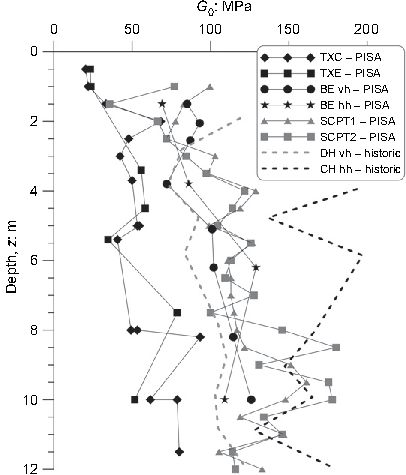
\includegraphics[width = 90mm]{Figures/figure-Cowden.pdf}
    \caption{Stiffness characteristics at Cowden from \protect\cite{zdravkovic2020}}
    \label{fig: Cowden_cpt}
\end{figure}






\section{Objectives and outlines}
\subsubsection{Objectives:}
This thesis aims to construct a robust and scalable framework for uncertainty quantification, extending its applicability beyond offshore piles. This endeavor will leverage cutting-edge methodologies in the fields of surrogate modeling, uncertainty quantification, probabilistic graphical model and control theory, to deliver a robust digital twin framework in geotechnical engineering. In particular, the specific goals of this research are:
\begin{itemize}[left=0pt]
    \item Develop a surrogate model suitable, not limited for offshore piles, for structures characterized by high input dimensions.
    
    \item Accelerate Bayesian inversion calculations for identified parameters to reduce the uncertainties, and providing real-time response predictions through adaptive enrichment of observed monitoring data.
    
    \item Develop an adaptive uncertainty quantification framework.

  
\end{itemize}


\subsubsection{Outlines:}
Chapter 2 introduces the fundamentals of Bayesian probabilistic theory.
Chapter 3 discusses the most important forward and inverse UQ tools.
Chapter 4 states the geotechnical UQ problems in our thesis and work plans for the next stage.

\chapter{State of the Art}

\label{ch:State}

\section{Markov Chain}

As shown in \cref{fig:fig2.1}, Markov Chain is involved in Bayesian inference calculation and can therefore reduce the analysis time and provide reasonable posterior results.


  \begin{figure}[htbp]
      \centering
       \begin{tikzpicture}[
              node distance=3cm,
              state/.style={circle, draw, fill=white, inner sep=0pt, minimum size=5mm},
              arrow/.style={->, >=latex, shorten >=1pt, thick}
            ]
              % Define state nodes
              \node[state] (X0) {$X_0$};
              \node[state, right of=X0] (X1) {$X_1$};
              \node[state, right of=X1] (X2) {$X_2$};
              \node[state, right of=X2] (Xdots) {$\dots$};
              \node[state, right of=Xdots] (Xn) {$X_n$};
            
              % Draw arrows
              \draw[arrow] (X0) -- node[above] {$P(X_1|X_0)$} (X1);
              \draw[arrow] (X1) -- node[above] {$P(X_2|X_1)$} (X2);
              \draw[arrow] (X2) -- node[above] {} (Xdots);
              \draw[arrow] (Xdots) -- node[above] {} (Xn);
            
              % Add time labels
              \node[below of=X0, node distance=0.8cm] (T0) {Time $t_0$};
              \node[below of=X1, node distance=0.8cm] (T1) {Time $t_1$};
              \node[below of=X2, node distance=0.8cm] (T2) {Time $t_2$};
              \node[below of=Xdots, node distance=0.8cm] (Tdots) {$\dots$};
              \node[below of=Xn, node distance=0.8cm] (Tn) {Time $t_n$};
            \end{tikzpicture}
              
      \caption{Markov Chain process}
      \label{fig:fig2.1}
  \end{figure}

  Markov Chain has two main features:
  \begin{itemize}
      \item State transition of Markov chains depends only on the current state, thus simplifying the modeling process
      \item Given the current state, a state transition probability distribution can be used to infer the likelihood of the next state

  \end{itemize}

  Thus, the properties of Markov Chain will bring two advantages: 

  \begin{itemize}
      \item Adapt to more complex models (with increasing soil parameters)
      \item Iterative updating of parameter estimates because of Markov Chain’s property (enables  updating the priors through Bayesian inference in stage)

  \end{itemize}


  \section{Partially observed Markov decision process (POMDP)}

As shown in \cref{fig:fig2.2}, based on Markov Chain, with introducing Rewards and Actions, it can form the basis of Partially observed Markov decision process.


\begin{figure}[htbp]
    \centering
    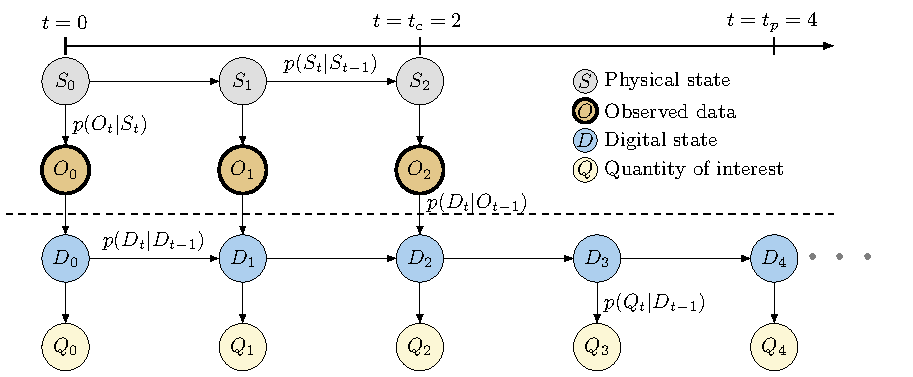
\includegraphics[width = 140mm]{Figures/figure3.pdf}
    \caption{Untrained strength profile at Cowden \protect\cite{kapteyn2021}}
    \label{fig:fig2.2}
\end{figure}


\section{Digital Twin}

Generally, Digital Twin can be divided into two main parts, including (1) calibration and assimilation (2) Prediction, as shown in \cref{equation 2.1}  and \cref{equation 2.2}.

\begin{equation}
\begin{aligned}
& p(D_{0},...,D_{t_{c}},Q_{0},...,Q_{t_{c}},R_{0},...,R_{t_{c}}|o_{0},...,o_{t_{c}},u_{0},...,u_{t_{c}}) \\
& = \prod_{t=0}^{t_{c}}[\phi_{t}^{update}\phi_{t}^{QoI}\phi_{t}^{evaluation}] \label{equation 2.1}
\end{aligned}
\end{equation}


\begin{equation}
\begin{aligned}
    & p(D_{0},...,D_{t_{p}},Q_{0},...,Q_{t_{p}},R_{0},...,R_{t_{p}},U_{t_{c}+1},...,U_{t_{p}}|o_{0},...,o_{t_{c}},u_{0},...,u_{t_{c}}) \\
    & \propto \prod_{t=0}^{t_{p}}[\phi_{t}^{dynamics}\phi_{t}^{QoI}\phi_{t}^{evaluation}] \prod_{t=0}^{t_{c}}\phi_{t}^{assimilation} \prod_{t=t_{c}+1}^{t_{p}}\phi_{t}^{control} \label{equation 2.2}
\end{aligned}
\end{equation}
\chapter{Active learning for Bayesian inference}

\section{Reduced-order surrogate model}

Computer modelling is used in nearly every field of science and engineering. Often, these computer codes model complex phenomena, have many input parameters,
and are expensive to evaluate. In order to explore the behavior of the model under uncertainty (e.g., uncertainty propagation, parameter calibration from data or sensitivity analysis), many
model runs are required. However, if the model is costly, only a few model evaluations can be afforded, which often do not suffice for thorough uncertainty quantification. In engineering and applied sciences, a popular work-around in this situation is to construct a reduced-order surrogate model. A reduced-order surrogate model is a cheap-to-evaluate proxy of the original model, which typically can be constructed from a relatively small number of model evaluations and approximates
the input-output relation of the original model well. Since the surrogate model is cheap to evaluate, uncertainty quantification can be performed at a low cost by using the surrogate
model instead of the original model. Therefore, surrogate modelling aims at constructing a metamodel that provides an accurate approximation to the original model while requiring as few model evaluations as possible for its construction.

\section{Bayesian inference framework}

\subsection{Bayes theorem for soil parameter estimate}

Bayesian theorem provides a possible tool to understand and update the uncertainties for the priors as shown in \cref{equation 1.1}.
\begin{equation}
P(A|B) = \frac{{P(B|A) \cdot P(A)}}{{P(B)}} \label{equation 1.1}
\end{equation}
$P(A|B)$: posterior: Distribution of soil parameters;$P(B|A)$:likelihood: observed data and FE simulation based on priors; $P(A)$: prior: Soil parameters from lab/field.

\subsection{Maximise a posterior estimation (MAP)}


\subsection{Sampling methods}

\subsection{Maximal likelihood estimation (MLE)}




\section{Sequential enrichment for surrogate model}

Instead of sampling the whole experimental design at once, it has been proposed to use sequential enrichment. Starting with
a small experimental design, additional points are chosen based on the last computed sparse
solution. In the context of machine learning, sequential sampling is also known as active learning.  In all
cases, numerical examples show that the sequential strategy generally leads to solutions with
a smaller validation error compared to non-sequential strategies



\section{Sequential Bayesian inference}







\chapter{A unified framework for digtital twins for piles}


This chapter develops a mathematical and computational foundation for digital twins of piles.




\section{Markov Chain}












As shown in \cref{fig:fig2.1}, Markov Chain is involved in Bayesian inference calculation and can therefore reduce the analysis time and provide reasonable posterior results.


  \begin{figure}[htbp]
      \centering
       \begin{tikzpicture}[
              node distance=3cm,
              state/.style={circle, draw, fill=white, inner sep=0pt, minimum size=5mm},
              arrow/.style={->, >=latex, shorten >=1pt, thick}
            ]
              % Define state nodes
              \node[state] (X0) {$X_0$};
              \node[state, right of=X0] (X1) {$X_1$};
              \node[state, right of=X1] (X2) {$X_2$};
              \node[state, right of=X2] (Xdots) {$\dots$};
              \node[state, right of=Xdots] (Xn) {$X_n$};
            
              % Draw arrows
              \draw[arrow] (X0) -- node[above] {$P(X_1|X_0)$} (X1);
              \draw[arrow] (X1) -- node[above] {$P(X_2|X_1)$} (X2);
              \draw[arrow] (X2) -- node[above] {} (Xdots);
              \draw[arrow] (Xdots) -- node[above] {} (Xn);
            
              % Add time labels
              \node[below of=X0, node distance=0.8cm] (T0) {Time $t_0$};
              \node[below of=X1, node distance=0.8cm] (T1) {Time $t_1$};
              \node[below of=X2, node distance=0.8cm] (T2) {Time $t_2$};
              \node[below of=Xdots, node distance=0.8cm] (Tdots) {$\dots$};
              \node[below of=Xn, node distance=0.8cm] (Tn) {Time $t_n$};
            \end{tikzpicture}
              
      \caption{Markov Chain process}
      \label{fig:fig2.1}
  \end{figure}

  Markov Chain has two main features:
  \begin{itemize}
      \item State transition of Markov chains depends only on the current state, thus simplifying the modeling process
      \item Given the current state, a state transition probability distribution can be used to infer the likelihood of the next state

  \end{itemize}

  Thus, the properties of Markov Chain will bring two advantages: 

  \begin{itemize}
      \item Adapt to more complex models (with increasing soil parameters)
      \item Iterative updating of parameter estimates because of Markov Chain’s property (enables  updating the priors through Bayesian inference in stage)

  \end{itemize}


  \section{Probabilistic graphical model of the
pile-digital twin system}

As shown in \cref{fig:fig2.2}, based on Markov Chain, with introducing Rewards and Actions, it can form the basis of Partially observed Markov decision process.


\begin{figure}[htbp]
    \centering
    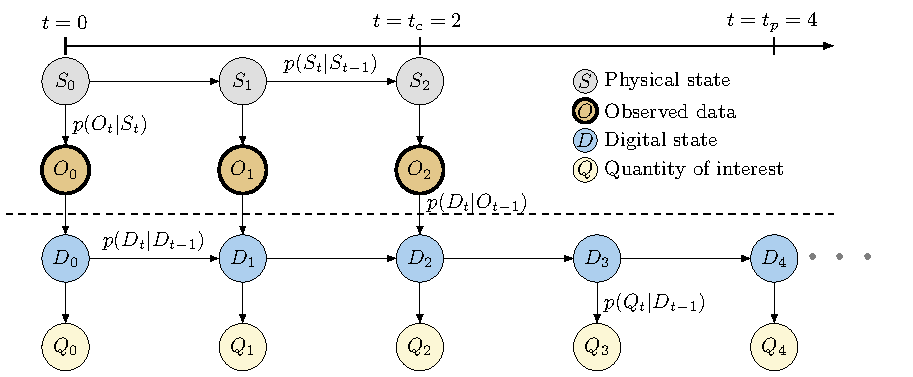
\includegraphics[width = 150mm]{Figures/figure3.pdf}
    \caption{Untrained strength profile at Cowden \protect\cite{kapteyn2021}}
    \label{fig:fig2.2}
\end{figure}



Generally, Digital Twin can be divided into two main parts, including (1) calibration and assimilation (2) Prediction, as shown in \cref{equation 2.1}  and \cref{equation 2.2}.

\begin{equation}
\begin{aligned}
& p(D_{0},...,D_{t_{c}},Q_{0},...,Q_{t_{c}},R_{0},...,R_{t_{c}}|o_{0},...,o_{t_{c}},u_{0},...,u_{t_{c}}) \\
& = \prod_{t=0}^{t_{c}}[\phi_{t}^{update}\phi_{t}^{QoI}\phi_{t}^{evaluation}] \label{equation 2.1}
\end{aligned}
\end{equation}


\begin{equation}
\begin{aligned}
    & p(D_{0},...,D_{t_{p}},Q_{0},...,Q_{t_{p}},R_{0},...,R_{t_{p}},U_{t_{c}+1},...,U_{t_{p}}|o_{0},...,o_{t_{c}},u_{0},...,u_{t_{c}}) \\
    & \propto \prod_{t=0}^{t_{p}}[\phi_{t}^{dynamics}\phi_{t}^{QoI}\phi_{t}^{evaluation}] \prod_{t=0}^{t_{c}}\phi_{t}^{assimilation} \prod_{t=t_{c}+1}^{t_{p}}\phi_{t}^{control} \label{equation 2.2}
\end{aligned}
\end{equation}




\section{Planning and prediction via digital twin}
\chapter{Focus of the Work}
\label{ch:Focus}

\section{Objectives}

Introduce Markov Chain process involving in Bayesian inverse analysis to reduce the inverse analysis time and provide reasonable posterior results for the soil parameters. Based on Markov Chain process, we also introduce the Reward function and Action function to form the basis of digital twin. Combined with monitored data, the proposed probabilistic graph model-Partially Observed Markov Decision Process can be used to mimic and predict the pile bearing behaviors.



\chapter{Work Plan}

\label{Work_Plan}

\section{Stage 1}
Calibrate the models in \cref{fig:fig-CM2pile} with partially observed Markov decision process.
\begin{figure}[H]
    \centering

    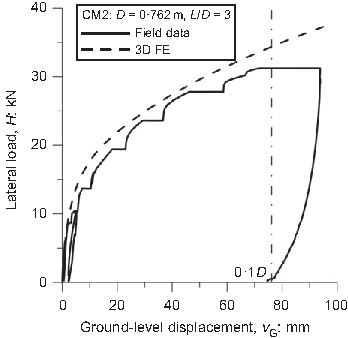
\includegraphics[width = 90mm]{Figures/figure-CM2.pdf}
    \caption{CM2 pile load displacement from \protect\cite{zdravkovic2020}}
    \label{fig:fig-CM2pile}
\end{figure}

\begin{itemize}
    \item Software: ICFEP-Likelihoods and observed data.
    \item Constitutive model: clay in \cite{zdravkovic2020} and sand in \cite{taborda2020}.
    \item Consider the soil profile variance-Create the random field (scale of fluctuation in ICFEP).
\end{itemize}
Objective: Ensure the soil parameters in digital model can reveal unique characteristics of piles.

\section{Stage 2}
In operational Phase, Based on Partially observed Markov decision process method, continue the assimilation process: extend the digital twin capability to capture the piles response during loading.

\section{Stage 3}
Extension to Prediction




\section{Time plan}
\begin{table}[h]
\caption{PhD timeline}
\vspace{10pt}
\centering
\resizebox{\textwidth}{!}{
\begin{tabular}{|l|l|l|l|l|l|l|l|l|l|l|l|l|l|l|l|l|l|}
\hline
month                                                                           & 0 & 3                     & 6 & 9 & 12 & 15 & 18 & 21 & 24 & 27 & 30 & 33 & 36 & 39 & 42 & 45 & 48 \\ \hline
Literature review                                                               & \checkmark &\checkmark               &\checkmark   &   &    &    &    &    &    &    &    &    &    &    &    &    &    \\ \hline
\begin{tabular}[c]{@{}l@{}}Numerical modelling\\ (Data collection)\end{tabular} &   &\checkmark&  \checkmark & \checkmark  & \checkmark   &\checkmark    & \checkmark   &    &    &    &    &    &    &    &    &    &    \\ \hline
\begin{tabular}[c]{@{}l@{}}Statistics Methods \\ learning\end{tabular}          &   &\checkmark                       &\checkmark   & \checkmark  &\checkmark    & \checkmark   &   \checkmark &\checkmark    &\checkmark    &    &    &    &    &    &    &    &    \\ \hline
\begin{tabular}[c]{@{}l@{}}Statistics analysis\\ calibration\end{tabular}       &   &                       & \checkmark  &  \checkmark & \checkmark   &    &    &    &    &    &    &    &    &    &    &    &    \\ \hline
\begin{tabular}[c]{@{}l@{}}Statistics analysis\\ assimilation\end{tabular}      &   &                       &   &   &    &  \checkmark  &   \checkmark &\checkmark    &  \checkmark  & \checkmark   &\checkmark    &    &    &    &    &    &    \\ \hline
\begin{tabular}[c]{@{}l@{}}Statistics analysis\\ prediction\end{tabular}        &   &                       &   &   &    &    &    &    &    &    &   &  \checkmark  &   \checkmark &  \checkmark   &    &    &    \\ \hline
Thesis writing                                                                  &   &                       &   &   &    &    &    &    &    &    &    &    &    &    &     \checkmark&  \checkmark   & \checkmark    \\ \hline
Journal/Conference                                                              &   &                       &   &   &    &    &    &     \checkmark&    &    &    &    \checkmark &    &    &    &    &  \checkmark   \\ \hline
\end{tabular}}
\end{table}

% body of thesis comes here

\input{conclusion/conclusion}

\appendix
% appendices come here


\addcontentsline{toc}{chapter}{Bibliography}
\bibliographystyle{apacite}
\bibliography{bibliography/bibliography}


\end{document}